\documentclass[11pt,letterpaper]{article}
\usepackage[T1]{fontenc}
\usepackage{fullpage}
\usepackage[top=2cm, bottom=4.5cm, left=2.5cm, right=2.5cm]{geometry}
\usepackage{amsmath,amsfonts,amssymb}
\usepackage{lastpage}
\usepackage[inline]{enumitem}
\usepackage{fancyhdr}
\usepackage{mathrsfs}
\usepackage{xcolor}
\usepackage{graphicx}
\usepackage{subcaption}
\usepackage{appendix}
\usepackage{hyperref}
\usepackage{titlesec}
\usepackage{fancyvrb}
\hypersetup{colorlinks=true, linkcolor=blue, linkbordercolor={0 0 1}}

%\renewcommand{\arraystretch}{1.5}
\titlespacing*{\section}{0pt}{0.65\baselineskip}{0.5\baselineskip}

\setlength{\parindent}{0.0in}
\setlength{\parskip}{0.05in}

\newcommand{\qrf}{\texttt{QRFactor}}

\pagestyle{fancyplain}
\lhead{}
\chead{GPU Solutions for PSCAD: IT17112}
\rhead{}
\cfoot{\small\thepage}
\headsep 32pt

%%%%%%%%%%%%%%%%%%%%%%%%%%%%%%%%%%%%%%%%%%%%%%%%%%%%%%%%%%%%%%%%%%%%%%%%%%%%%%%
%%%%%%%%%%%%%%%%%%%%%%%%%%%%%%%%%%%%%%%%%%%%%%%%%%%%%%%%%%%%%%%%%%%%%%%%%%%%%%%

\begin{document}
\begin{center}
    {\Large \bf Monthly Summary: November, 2020}
\end{center}

\section*{\texttt{QRFactor.cpp}}

This month, development and documentation of the GPU/PSCAD interface \verb+QRFactor.cpp+ was completed -- see appendix~\ref{sec: header file} for documentation. We successfully created a QRFactor class with host-based sparse matrix construction and device-based matrix factoring and solving. We tested this code with several small examples and checked the results against host-only solving methods; in all cases the results from the two methods agreed. Custom error codes were created and documented to aide in later debugging of QRFactor within a larger program -- see appendix~\ref{sec: Error Codes} for these definitions.

The final version of this code did not rely on direct memory copying. Instead, the Eigen sparse matrix object was used to generate the CSR pointers during the factoring process, after which they are not needed and are allowed to go out of scope. The essential class members that hold the result of factoring the sparse matrix are: (size\verb+_+t) \verb+msize_factor+, (csrprinfo\verb+_+t) \verb+m_info+, (cusolverSpHandle\verb+_+t) \verb+m_cusolverSpH+, and (cudaStream\verb+_+t) \verb+m_stream+. After being calculated by the device-side function \verb+__host__ __device__ void QRFactor::factor()+, these variables are called during all subsequent uses of the device-side function \verb+__host__ __device__ void QRFactor::solve(bvector, xvector)+. While this version of QRFactor did successfully separate the GPU-based solving code into functions that could be called from another program, a more useful packaging of the solution was needed for better integration into existing PSCAD software.

\section*{\texttt{QRFactorLib.dll}}

After discussions with MHI, it was decided that the development of a Dynamic Link Library (DLL) for \qrf\! was the next major goal. A step-by-step guide for creating and using DLLs within Microsoft Visual Studio 2019 can be found in the \href{https://docs.microsoft.com/en-us/cpp/build/walkthrough-creating-and-using-a-dynamic-link-library-cpp?view=msvc-160#see-also}{Microsoft C/C++ projects documentation}. Creating a DLL for QRFactor will allow for the easiest integration into PSCAD, however the structure of DLLs differs significantly from a regular EXE program and so some restructuring is required. 

In particular, any classes or functions that are accessible to the client program ({\it i.e.}, the program importing the DLL) can only use primitive data types. Because \qrf\! relies on data types derived from the vector STL and Eigen headers, some level of obfuscation must be employed. To accomplish this, separate classes for the Eigen sparse matrix and Eigen triplets were written. Pointers to instances of these classes were included in the QRFactor class, thereby satisfying the primitive data type requirement. See figure~\ref{fig: class diagram} for a diagram of how these classes relate to one another. It should be noted that the Sparse class is derived from the Coefficients base class.

\begin{figure}[h]
    \centering
    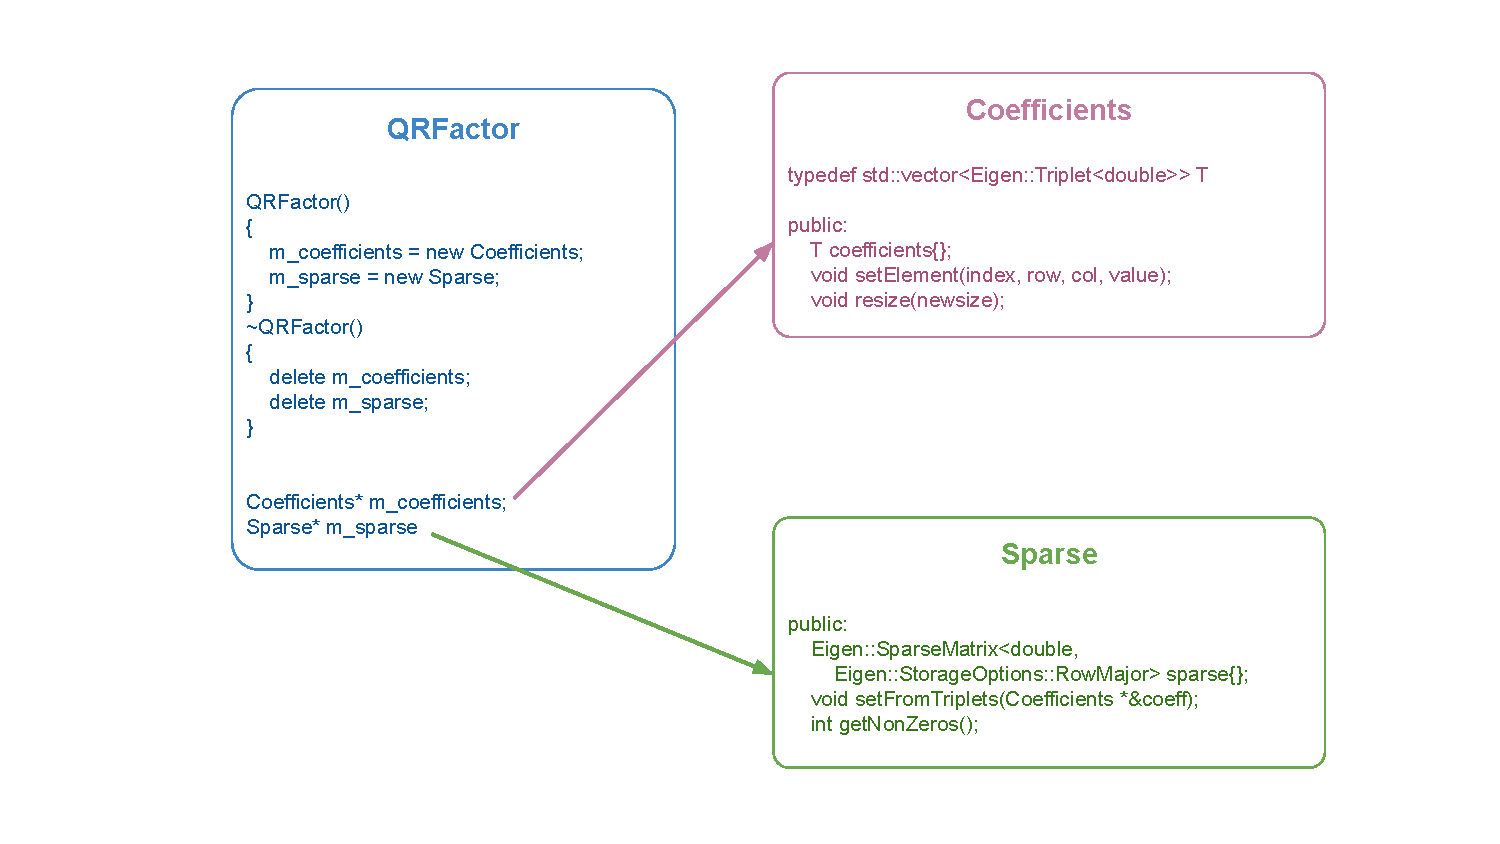
\includegraphics[width=0.8\textwidth]{QRFactorLib_Diagram.pdf}
    \caption{A diagram of the Dynamic Link Library structure of QRFactor. The Coefficients and Sparse classes are defined in their own header files and only pointers to these classes are included in the exported class.}
    \label{fig: class diagram}
\end{figure}

Currently, all host-only functions and variables have been incorporated into the QRFactor DLL and client testing has confirmed that it is functioning properly. During the month of December, CUDA variables and device-side functions will be incorporated into the QRFactor DLL. This requires employing the NVIDIA compiler \verb+nvcc+ in the place of the Microsoft Visual C++ compiler during DLL creation. It remains to be seen if additional changes to the development template used by Visual Studio for DLL creation will be required.

\appendix
\section*{}
\section{\texttt{QRFactor.h}}
\label{sec: header file}
\begin{verbatim}

/*
* QRFactor.h
* --------------------------------------------------------------------------
* --------------------------------------------------------------------------
* This header provides tools for interfacing between GPU-based, sparse
* matrix solving methods and PSCAD/EMTDC software
* 
* Created by:
* Brad Cownden <cowndenb@gmail.com> 
* as part of MITACS Industrial Postdoc Award IT17112
* 
* To be included with this header is the open source Eigen template library 
* that provides methods for sparse matrix descriptions on the host:
* http://eigen.tuxfamily.org
* --------------------------------------------------------------------------
* --------------------------------------------------------------------------
*/


#pragma once
#include <vector>			  // Storage of the list of non-zero matrix values
#include <Eigen/SparseCore>	  // Eigen sparse library

#include "cusolverSp.h"		  // CUDA sparse solving library
#include <cuda_runtime.h>	  // __host__ and __device__
#include "helper_cuda.h"	  // Checking cuda errors

/*
* Documentation
* --------------------------------------------------------------------------
* --------------------------------------------------------------------------
* QRFactor (Class)
* --------------------------------------------------------------------------
* --------------------------------------------------------------------------
* Members:
* 
*	m_rowsA 
*		Type: size_t
*		Description: the number of rows of the total system matrix, A.
* 
*	m_colsA
*		Type: size_t
*		Description: the number of columns of the total system matrix, A. Note
*					 that m_colsA == m_rowsA in EMTDC data, although this need
*					 not be true for general data.
*	
*	m_rowOffset
*		Type: int
*		Description: during the build of the full system matrix by reading 
*					 multiple, dense submatrices this index tracks the row
*					 offset from (0,0) to the current submatrix, ensuring that
*					 each submatrix is added to the full system matrix along
*					 the diagonal.
* 
*	m_colOffset
*		Type: int
*		Description: this index plays the same role as m_rowOffset, but for
*					 the number of columns. In most EMTDC applications, this
*					 will be equal to m_rowOffset.
* 
*	m_nnzA
*		Type: size_t
*		Description: the number of non-zero values in the full system sparse
*					 matrix.
* 
*	m_coefficients
*		Type: std::vector<Eigen::Triplet<double>>
*		Description: this vector stores the non-zero entries from each dense
*					 submatrix as it is read in. The format of the 
*					 Eigen::Triplet object is (i, j, value) where i is the
*					 row number, j is the column number, and value is the
*					 entry in the matrix. Triplets do not need to be entered
*					 in any particular order. Using the Eigen method
*					 setFromTriplets(), a sparse matrix in compressed form
*					 is created from the triplets.
* 
*	m_sparse
*		Type: Eigen::SparseMatrix
*		Description: this object describes a sparse matrix of doubles with Row-
*					 Major ordering (Eigen sparse matrices are Column-Major by
*					 default). It is created out of the triplets in
*					 m_coefficients using Eigen::setFromTriplets and stores
*					 information such as the size of the matrix, the non-zero
*					 entries, as well as providing methods for extracting the
*					 compressed storage, row-major description of the matrix 
*					 in terms of three CSR pointers. See the CUDA cuSparse
*					 documentation on compressed storage descriptions:
*					 https://docs.nvidia.com/cuda/cusparse/index.html
*
*	msize_factor
*		Type: size_t
*		Description: the size factor determined by cusolverSpDcsrqrBufferInfo()
*					 that is required to create a buffer of total size
*					 sizeof(char) * msize_factor on the GPU where factoring
*					 and solving will take place.
* 
*	m_info
*		Type: csrqrInfo_t
*		Description: this opaque CUDA object is part of the cuSolverSp library
*					 that contains all the information about the sparse matrix
*					 A, stored in CSR format and factored using QR methods.
*					 It is initially used during the factoring phase, after
*					 which it is used repeatly as read-only data during the 
*					 solving phase of the algorithm. See the CUDA cuSolverSp
*					 documentation for more information:
*					 https://docs.nvidia.com/cuda/cusolver/index.html.
*					 
*	m_cusolverSpH
*		Type: cusolverSpHandle_t
*		Description: this is a pointer type to an opaque cuSolverSp context
*					 that must be passed to every cuSolverSp function. See the
*					 CUDA cuSolverSp documentation for more information:
*					 https://docs.nvidia.com/cuda/cusolver/index.html.
* 
*	m_stream
*		Type: cudaStream_t
*		Description: a stream is a sequence of commands that execute in order,
*					 and may possibly contain commands from different host
*					 threads. If no stream is specified, the default stream
*					 between the host and device is used. However, data and
*					 commands going to and from the device can be overlapped
*					 through the use of streams. In this case, an explicit
*					 stream is created to pass m_cusolverSpH between the host
*					 and the device. If data transfer become a limiting 
*					 factor in performance, separate streams for data and
*					 m_cusolverSpH could be created and overlapped.
* --------------------------------------------------------------------------
* --------------------------------------------------------------------------
* Methods:
* 
*	void buildTriplets
*		(
*			const double* inputArr,
*			const int rows,
*			const int cols
*		)
* 
*		Parameters:
*			inputArr
*				Type: (const double*)
*				Description: a pointer to an array of doubles that give the
*							 column-major description of a dense subsystem. 
*							 The array will have (rows * cols) entries.
*			rows
*				Type: const int
*				Description: the number of rows in the dense subsystem.
*			cols
*				Type: const int
*				Description: the number of columns in the dense subsystem.
* 
*		Return value:
*			No return value
*			Description: the non-zero values of inputArr are stored in the
*						 vector of triplets m_coefficients to be used later
*						 when constructing m_sparse. The values of m_rowOffset
*						 and m_colOffset are incremented such that
*						 m_rowOffset += rows and m_colOffset += cols after the
*						 non-zero values have been added to m_coefficients.
* 
*		Remarks:
*			This function is called repeatedly as all the subsystems are
*			gathered to create the full system sparse matrix, A. Ideally, this
*			step could be eliminated by bypassing subsystem splitting if it is
*			determined ahead of time that the system is large enough to
*			benefit from running on the GPU. 
*			The triplets (i, j, value) give the row and column position 
*			within the entire system matrix of the entry value. Therefore, 
*			after the data from inputArr has been read in, the internal values
*			m_rowOffset and m_colOffset must be incremented so that the next
*			array to be read in will always be along the diagonal of the full
*			system matrix.
*			Internal to this function is a call to the std::vector function
*			resize() that increases the size of the vector m_coefficients so
*			that new values can be read in. For memory efficiency, the number
*			of non-zero entries in inputArr is counted first so that
*			m_coefficients can be resized a single time. As a check, the 
*			previous size of m_coefficients is kept in a temporary variable
*			and incremented with each triplet addition. An if condition
*			ensures that entries in m_coefficients are not overwritten, and
*			there is not an attempt to access memory past the end of the
*			vector.
* 
*		Example:
*			// Create the QRFactor object
*			QRFactor qr;
*			// Add the non-zero values from a 3x3 dense subsystem matrix 
*			// in colum-major order
*			double dense_subsys[9] = { 1.0, 0.0, 2.0, 
*									   3.0, 4.0, 5.0, 
*									   6.0,	0.0, 7.0 };
*			double* inputPtr;
*			inputPtr = dense_subsys;
*			int rows { 3 };
*			int cols { 3 };
*			
*			// Add non-zero values to list of triplets
*			qr.buildTriplets(inputPtr, rows, cols);
*
*			// Given another pointer to an array for the values of a 4x4
*			// dense subsystem matrix in column-major order, add the non-zero
*			// values to the full system sparse matrix
*			qr.buildTriplets(anotherPtr, 4, 4);		
*
* --------------------------------------------------------------------------
*	
*	void buildSparseMatrix
*		(
*			void
*		)
* 
*		Parameters:
*			No parameters
*
*		Return value:
*			No return value
*
*		Remarks:
*			Once all the non-zero values from all the submatrices have been
*			read in to m_coefficients, the sparse matrix m_sparse can be
*			constructed using existing Eigen methods. Within this function, 
*			the memory reserved for the sparse matrix is set with a call to
*			m_sparse.resize(), before the triplets containing the coordinates
*			and values of the non-zero entries are given to m_sparse via
*			setFromTriplets(), which takes start and end iterators as inputs.
*			Once the triplets have been read in, the memory used to store the
*			matrix is minimized by calling the Eigen methods data().squeeze().
*			The final step of creating the sparse matrix is to extract the
*			number of non-zero entries (m_nnzA), number of rows (m_rowsA), and
*			number of columns (m_colsA) so that these can be used elsewhere
*			in the program.
*			This step also implicitly defines the CSR pointers outerIndexPtr,
*			innerIndexPtr, and valuePtr that are required for factoring on the
*			device.
* 
*		Example:
*			// Create the QRFactor object
*			QRFactor qr;
* 
*			// Read in dense subsystems
*			.
*			.
*			.
* 
*			// All subsystems have been read in. Create sparse matrix A
*			qr.buildSparseMatrix()
* 
* --------------------------------------------------------------------------
* 
*	__host__ __device__ void factor
*		(
*			void
*		)
* 
*		Parameters:
*			No parameters
* 
*		Return value:
*			No return value
* 
*		Remarks:
*			This function is decorated with __host__ __device__ so that nvcc
*			will compile a version to run on the GPU that can be called by
*			the host.
*			This function performs the one-time factoring of the full, sparse
*			system matrix using low-level CUDA libraries. Once this function
*			has been called, the result of the QR decomposition will be stored
*			in class members that can quickly and repeatedly be used to solve
*			the linear system Ax=b. A description of the QR method can be
*			found here: https://en.wikipedia.org/wiki/QR_decomposition
*			An outline of the process involved in QR decomposition in the GPU
*			is as follows: 
*				-- Create host and device pointers for the CSR
*				   description of the system matrix A
*				-- Fill host pointers with CSR description provided by Eigen
*				-- Create matrix handle and information to store the result of
*				   the factoring and to be used in all matrix operatorions
*				-- Send the host pointers to the device
*				-- Use low-level cuSolverSp methods to set up and compute the
*				   factored version of A, which is stored in the class members
*				   m_cusolverSpH and m_info
*			A functional example of low-level QR factoring using CUDA can be
*			found in 7_CUDALibraries/cuSolverSp_LowlevelQR in the CUDA Samples
*			directory.
* 
*		Example:
*			// Create the QRFactor object
*			QRFactor qr;
* 
*			// Read in all the dense subsystems 
*			.
*			.
*			.
* 
*			// Make the sparse system matrix
*			qr.buildSparseMatrix();
* 
*			// Factor on the device
*			qr.factor();
* 
* --------------------------------------------------------------------------
*
*	__host__ __device__ void solve
*		(
*			const double* bVector,
*			double*& xVector
*		)
* 
*		Parameters:
*			bVector
*				Type: const (double*)
*				Description: a pointer to doubles that make up the right hand 
*							 side vector, b, in the equation Ax=b
* 
*			xVector
*				Type: double*&
*				Description: a reference to a pointer of doubles that will
*							 hold the result vector, x, in the equation Ax=b
* 
*		Return value:
*			No return value
* 
*		Remarks:
*			This function is decorated with __host__ __device__ so that nvcc
*			will compile a version to run on the GPU that can be called by
*			the host.
*			This function uses the factored version of the sparse matrix A to
*			solve the linear equation Ax=b for x given the right hand side
*			solution vector b. Note that factor() must have already been
*			called so that m_cusolverSpH and m_info contain the factored
*			version of A. This function can be called repeatedly once the QR
*			form of A has been determined. The solution vector is stored in 
*			the input vector xVector.
*
* 
*		Example:
*			// Assume that the object qr has been properly factored and is 
*			// ready to be used to solve the equation Ax=b. Let the dimensions
*			// of A be 10x10, so that the vectors b and x must also have
*			// lengths of 10
* 
*			// Input and solution vectors
*			double* b = { 0.0, 1.0, 2.0, ...,9.0 };
*			double* x = NULL;
*			x = (double*)malloc(sizeof(double) * 10);
* 
*			// Use factored matrix to solve for x
*			qr.solve(const_cast<double*>(b), x);
* 
*			// x now contains the solution to the linear equation
* 
* --------------------------------------------------------------------------
* --------------------------------------------------------------------------
*/

class QRFactor
{
	typedef Eigen::Triplet<double> T; // Shorthand for Eigen triplet type

public:

	__host__ QRFactor() = default; 

	/*
	* Main factoring and solving functions
	*/
	__host__ __device__ void factor();
	__host__ __device__ void solve(const double* bVector, double*& xVector);
	
	/*
	* Building sparse matrix
	*/
	void buildTriplets(const double* inputArr, const int rows, const int cols);
	void buildSparseMatrix();
	
	/*
	* Destructor
	*/ 
	~QRFactor()
	{
		if (m_cusolverSpH) { checkCudaErrors(cusolverSpDestroy(m_cusolverSpH)); }
		if (m_stream) { checkCudaErrors(cudaStreamDestroy(m_stream)); }
		if (m_info) { checkCudaErrors(cusolverSpDestroyCsrqrInfo(m_info)); }
	}

private:

	size_t m_rowsA{ 0 };
	size_t m_colsA{ 0 };
	int m_rowOffset{ 0 };
	int m_colOffset{ 0 };
	size_t m_nnzA{ 0 };

	// Vector of Eigen triplets
	std::vector<T> m_coefficients;	
	// Eigen matrices are column-major by default, want row-major
	Eigen::SparseMatrix<double, Eigen::StorageOptions::RowMajor> m_sparse{}; 

	/*
	* CUSOLVER/CUSPARSE variables 
	*/
	size_t msize_factor = 0;		
	csrqrInfo_t m_info = NULL;
	cusolverSpHandle_t m_cusolverSpH = NULL;
	cudaStream_t m_stream = NULL;
	
};
\end{verbatim}

\section{\texttt{QRFactor Error Codes}}
\label{sec: Error Codes}

\begin{verbatim}
    /*
    * QRError.cpp
    *
    * Error codes used in QRFactor
    */

    #include <iostream>		// std::cerr
    #include "QRError.h"
    
     void getQRFactorError(QRFactor_Error &error)
    {
         // Given the error code, return a description of what raised the error
    
         switch (error)
         {
         case QRFactor_Error::SUCCESS:
             break;
         case QRFactor_Error::SINGULARITY_ERROR:
             std::cerr << "\nERROR: system matrix A is not invertible\n";
             break;
         case QRFactor_Error::SIZE_ERROR:
             std::cerr << "\nERROR: system matrix A must be square\n";
             break;
         case QRFactor_Error::BAD_BUFFER_SOLVE:
             std::cerr << "\nERROR: Working buffer could not be allocated in solve()\n";
             break;
         case QRFactor_Error::BAD_BUFFER_FACTOR:
             std::cerr << "\nERROR: Working buffer could not be allocated in factor()\n";
             break;
         default:
             std::cerr << "\nUnrecognized QRFactor class error\n";
             break;
         }
    
         error = QRFactor_Error::SUCCESS;
    
    }
    
\end{verbatim}


%%%%%%%%%%%%%%%%%%%%%%%%%%%%%%%%%%%%%%%%%%%%%%%%%%%%%%%%%%%%%%%%%%%%%%%%%%%%%%%
%%%%%%%%%%%%%%%%%%%%%%%%%%%%%%%%%%%%%%%%%%%%%%%%%%%%%%%%%%%%%%%%%%%%%%%%%%%%%%%































\end{document}
